\documentclass[tikz,border=5pt]{standalone}
\usepackage[UTF8]{ctex}
\usepackage{amsmath,amssymb}
\usetikzlibrary{arrows.meta,calc,angles,quotes,patterns,decorations.pathmorphing}
\definecolor{field}{HTML}{176B9B}
\definecolor{force}{HTML}{B64B32}
\tikzset{>=Latex,line width=.8pt,every node/.style={font=\small},field/.style={color=field},force/.style={color=force},body/.style={draw=black,fill=blue!5},ghost/.style={dashed,gray},labelbox/.style={fill=white,inner sep=1.2pt}}
\begin{document}
\begin{tikzpicture}
\draw[->](-1.1,0)--(4.7,0)node[right]{$z$};
\fill[force](-.25,0)circle(2pt)node[below]{$-$};
\fill[field](.25,0)circle(2pt)node[below]{$+$};
\draw[->,field](-.5,-.65)--(.7,-.65)node[right]{$\boldsymbol p$};
\draw[ghost](3,1.5)arc(90:270:.6 and 1.5);
\draw[thick](3,-1.5)arc(270:450:.6 and 1.5);
\fill[force](3.4596,.9642)circle(2.8pt)node[right]{$-q,m$};
\draw[->,field](3.4596,.9642)--(3.19,1.48)node[above]{$\boldsymbol v$};
\draw(3,0)--(3,1.5)node[midway,left]{$a$};
\draw[<->](0,-2)--(3,-2)node[midway,below]{$z_0$};
\draw[ghost](0,0)--(0,-2);\draw[ghost](3,0)--(3,-2);
\end{tikzpicture}
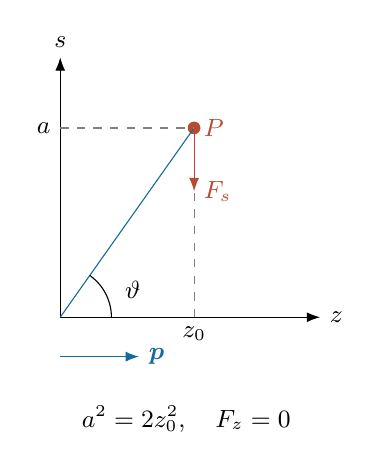
\begin{tikzpicture}
\draw[->](0,0)--(3.3,0)node[right]{$z$};
\draw[->](0,0)--(0,3.3)node[above]{$s$};
\coordinate(P)at(1.7,2.404);\fill[force](P)circle(2.3pt)node[right]{$P$};
\draw[field](0,0)--(P);
\draw[ghost](1.7,0)--(P);\draw[ghost](0,2.404)--(P);
\draw[->,force](P)--(1.7,1.6)node[right]{$F_s$};
\draw[->,field](0,-.5)--(1,-.5)node[right]{$\boldsymbol p$};
\draw(.65,0)arc(0:54.7356:.65);
\node[right]at(.7,.35){$\vartheta$};
\node[below]at(1.7,0){$z_0$};\node[left]at(0,2.404){$a$};
\node[below]at(1.6,-1){$a^2=2z_0^2,\quad F_z=0$};
\end{tikzpicture}
\begin{tikzpicture}
\draw[->](0,0)--(4.5,0)node[right]{$z$};
\draw[->](0,0)--(0,3.2)node[above]{$s$};
\draw[thick](.7,2)--(4,2)node[right]{绝缘杆};
\fill(1.8,2)circle(2.2pt)node[above left]{平衡点};
\fill[force](2.8,2)circle(2.6pt)node[above]{$P'$};
\draw[<->](1.8,1.5)--(2.8,1.5)node[midway,below]{$\eta>0$};
\draw[->,force,thick](2.8,2)--(2.15,2)node[midway,below=3pt]{$F_z<0$};
\draw[ghost](0,2)--(.7,2);\node[left]at(0,2){$a$};
\draw[ghost](1.8,0)--(1.8,2);\node[below]at(1.8,0){$z_0$};
\end{tikzpicture}
\begin{tikzpicture}
\begin{scope}
\draw[ghost](0,0)circle(1.25);
\fill(0,0)circle(1.5pt)node[below left]{轴};
\fill[force](1.7,0)circle(2.4pt)node[below right]{$s=a+\xi$};
\draw[->,force](1.7,0)--(.9,0)node[midway,below]{$F_{\rm eff}$};
\draw[->,field](1.7,0)--(1.7,.9)node[above]{$v_\phi$};
\draw(0,0)--(1.25,0)node[midway,above]{$a$};
\node[below]at(.2,-1.8){固定 $z_0$，$\ell=msv_\phi$ 守恒};
\end{scope}
\begin{scope}[xshift=4.2cm]
\draw[->](0,0)--(3.5,0)node[right]{$s$};
\draw[->](0,0)--(0,2.6)node[above]{$U_{\rm eff}$};
\draw[field,thick,domain=.68:1.5,samples=60]plot({2*\x},{18*(.38490018/(\x*\x)-.70710678/((\x*\x+.5)^1.5))});
\fill[force](2,0)circle(2pt)node[below]{$a$};
\node[below]at(1.8,-1.8){圆轨道是局部最低点};
\end{scope}
\end{tikzpicture}
\end{document}

